\documentclass[11pt,a4paper]{article}
% Preambulo comun de los reportes de Tecnologias Celulares.
% Cada main.tex hace: \documentclass ... \input{../comun/preambulo.tex}
\usepackage[utf8]{inputenc}
\usepackage[T1]{fontenc}
\usepackage[spanish,mexico]{babel}
\usepackage{graphicx}
\usepackage[margin=2.5cm]{geometry}
\usepackage{amsmath}
\usepackage{amssymb}
\usepackage{booktabs}
\usepackage{tabularx}
\usepackage{array}
\usepackage{float}
\usepackage{setspace}
\usepackage{parskip}
\usepackage{fancyhdr}
\usepackage{textcomp}
\usepackage{xcolor}
\usepackage{caption}
\usepackage{fvextra}
\usepackage[hidelinks]{hyperref}

\onehalfspacing
\setlength{\parskip}{6pt}
\sloppy
\setlength{\emergencystretch}{3em}
\setlength{\headheight}{40pt}
\captionsetup{font=small,labelfont=bf}
\setlength{\tabcolsep}{6pt}

\pagestyle{fancy}
\fancyhf{}
\fancyhead[L]{\includegraphics[width=1cm]{/home/yovick/repos/UAZ-IEI/Assets/UIE.png}}
\fancyhead[R]{\small Tecnologías Celulares}
\fancyfoot[C]{\thepage}
\renewcommand{\headrulewidth}{0.4pt}

\DefineVerbatimEnvironment{codigo}{Verbatim}{%
  breaklines=true,breakanywhere=true,fontsize=\small,frame=single,
  framesep=3pt,rulecolor=\color{gray!50}}

% Figura centrada con pie: \figura[ancho]{archivo}{leyenda}
\newcommand{\figura}[3][0.85]{%
  \begin{center}
    \includegraphics[width=#1\linewidth]{#2}\\[2pt]
    {\small #3}
  \end{center}}

% Portada: \portada{numero}{titulo de la practica}
\newcommand{\portada}[2]{%
\begin{titlepage}
  \thispagestyle{empty}
  \begin{center}
    \vspace*{1cm}
    \includegraphics[width=4.5cm]{/home/yovick/repos/UAZ-IEI/Assets/uaz.png}
    \vspace{0.8cm}

    {\large Universidad Autónoma de Zacatecas}\\[4pt]
    {\large Unidad Académica de Ingeniería Eléctrica}\\[4pt]
    {\normalsize Ingeniería Electrónica Industrial con especialidad en Telecomunicaciones}

    \vspace{1.8cm}
    {\LARGE\bfseries Práctica #1}\\[10pt]
    {\Large\bfseries #2}
  \end{center}

  \vspace{2.2cm}
  \begin{center}
    \begin{tabular}{rl}
      \textbf{Materia:} & Tecnologías Celulares\\
      \textbf{Docente:} & Dr. Víktor Iván Rodríguez Abdalá\\
      \textbf{Alumno:}  & Arnold Yovick Ríos Zaldívar\\
      \textbf{Fecha:}   & Noviembre de 2026\\
    \end{tabular}
  \end{center}
  \vfill
\end{titlepage}}

\usepackage{listings}

\graphicspath{{figs/}}

% Los numeros de seccion de dos cifras no caben en el ancho por omision del indice.
\makeatletter
\renewcommand{\l@section}{\@dottedtocline{1}{0em}{2.4em}}
\makeatother

% Listado de codigo leido directamente del archivo .m (siempre sincronizado).
\newcommand{\listado}[1]{%
  \VerbatimInput[fontsize=\scriptsize,breaklines=true,breakanywhere=true,
    frame=single,framesep=2pt,rulecolor=\color{gray!50},numbers=left,
    numbersep=4pt]{#1}}

\begin{document}

% ---------------------------------------------------------------- portada
\begin{titlepage}
  \thispagestyle{empty}
  \begin{center}
    \vspace*{1cm}
    \includegraphics[width=4.5cm]{/home/yovick/repos/UAZ-IEI/Assets/uaz.png}
    \vspace{0.8cm}

    {\large Universidad Autónoma de Zacatecas}\\[4pt]
    {\large Unidad Académica de Ingeniería Eléctrica}\\[4pt]
    {\normalsize Ingeniería Electrónica Industrial con especialidad en Telecomunicaciones}

    \vspace{1.8cm}
    {\LARGE\bfseries Tarea 2}\\[10pt]
    {\Large\bfseries Espectro disperso: simulaciones Monte Carlo}
  \end{center}

  \vspace{2.2cm}
  \begin{center}
    \begin{tabular}{rl}
      \textbf{Materia:}   & Tecnologías Celulares\\
      \textbf{Docente:}   & Dr. Víktor Iván Rodríguez Abdalá\\
      \textbf{Alumno:}    & Arnold Yovick Ríos Zaldívar\\
      \textbf{Matrícula:} & 35167151\\
      \textbf{Grupo:}     & VII\\
      \textbf{Fecha:}     & Noviembre de 2026\\
    \end{tabular}
  \end{center}
  \vfill
\end{titlepage}

\tableofcontents
\newpage

% ------------------------------------------------------------ introduccion
\section{Introducción}

Esta tarea resuelve los once problemas de simulación del capítulo de espectro
disperso: sistemas DS/SS sobre ruido blanco, detección de señales de baja
probabilidad de interceptación, secuencias de longitud máxima y secuencias Gold,
acceso múltiple por código (CDMA) síncrono y asíncrono, y sistemas de salto de
frecuencia (FH) con interferencia de banda parcial y diversidad.

Todos los programas están escritos en MATLAB y se ejecutaron con GNU Octave
(compatible con MATLAB en la sintaxis empleada), porque el equipo no cuenta con
licencia de MATLAB. Cada script fija su semilla, guarda sus figuras en
\texttt{figs/} y sus resultados numéricos en \texttt{datos/}, de modo que las
cifras citadas en este reporte se pueden reproducir con
\begin{center}
\texttt{octave --no-gui problemaNN.m}
\end{center}
desde la carpeta \texttt{tarea2/}. Las funciones compartidas (generación de
secuencias, autocorrelación y motores de simulación) están en \texttt{comun/} y
se listan en el apéndice~\ref{ap:comun}.

\paragraph{Notación.} $L$ es el número de chips por bit (ganancia de
procesamiento $G_p=L$), $E_c$ la energía por chip, $E_b=L\,E_c$ la energía por
bit, $N_0/2$ la densidad espectral de potencia del ruido blanco y
$Q(x)=\tfrac12\operatorname{erfc}(x/\sqrt2)$ la función gaussiana complementaria.
La autocorrelación periódica de una secuencia bipolar $c_n\in\{-1,+1\}$ se
calcula, como en la ecuación (20) del texto, con
\begin{equation}
  R_c(\tau)=\frac{1}{L}\sum_{n=1}^{L} c_n\,c_{n+\tau},
  \qquad c_{n+L}=c_n,
  \label{eq:autocorr}
\end{equation}
de manera que $R_c(0)=1$. En todos los casos la BER se estima como la fracción
de bits decididos incorrectamente en una simulación Monte Carlo.

% ------------------------------------------------------------- problema 1
\section{Problema 1: DS/SS binario sobre un canal AWGN}

\begin{quote}
\itshape
Escriba un programa de MATLAB para realizar una simulación Monte Carlo de un
sistema de espectro disperso DS que transmita la información vía PSK binario a
través de un canal AWGN. Suponga que la ganancia de procesamiento es 10.
Grafique la tasa de error medida vs el SNR y, así, demuestre que no hay ganancia
de desempeño a partir de la señal de espectro disperso.
\end{quote}

\paragraph{Modelo.} El transmisor multiplica los datos $d(t)=\pm1$ por un código
PN $c(t)=\pm1$ de $L=10$ chips por bit y modula en BPSK:
\begin{equation}
  s(t)=\sqrt{2E_c}\,d(t)\,c(t)\cos(2\pi f_c t),\qquad E_c=E_b/L.
\end{equation}
El receptor correlaciona con su réplica del código y con la portadora. La
variable de decisión para un bit vale
\begin{equation}
  y=\sqrt{E_c}\,L\,d+n,\qquad \sigma_n^2=L\,\frac{N_0}{2},
\end{equation}
por lo que la relación señal a ruido después del desensanchamiento es
\begin{equation}
  \mathrm{SNR}_\text{out}=\frac{(L\sqrt{E_c})^2}{L N_0/2}=\frac{2E_b}{N_0},
\end{equation}
exactamente la de BPSK sin dispersión. La probabilidad de error teórica es
$P_e=Q\!\left(\sqrt{2E_b/N_0}\right)$.

\paragraph{Método.} Se simularon $N=200\,000$ bits para cada valor de $E_b/N_0$
entre 0 y 8 dB, con un código aleatorio fijo de 10 chips y ruido gaussiano por
chip. La simulación se implementó en forma vectorizada
(\texttt{comun/sim\_dsss.m}).

\paragraph{Resultados.} La figura~\ref{fig:p01} y la tabla~\ref{tab:p01}
comparan la BER medida con la teoría de BPSK. Las dos curvas coinciden dentro
del error estadístico de la simulación.

\begin{figure}[H]
  \centering
  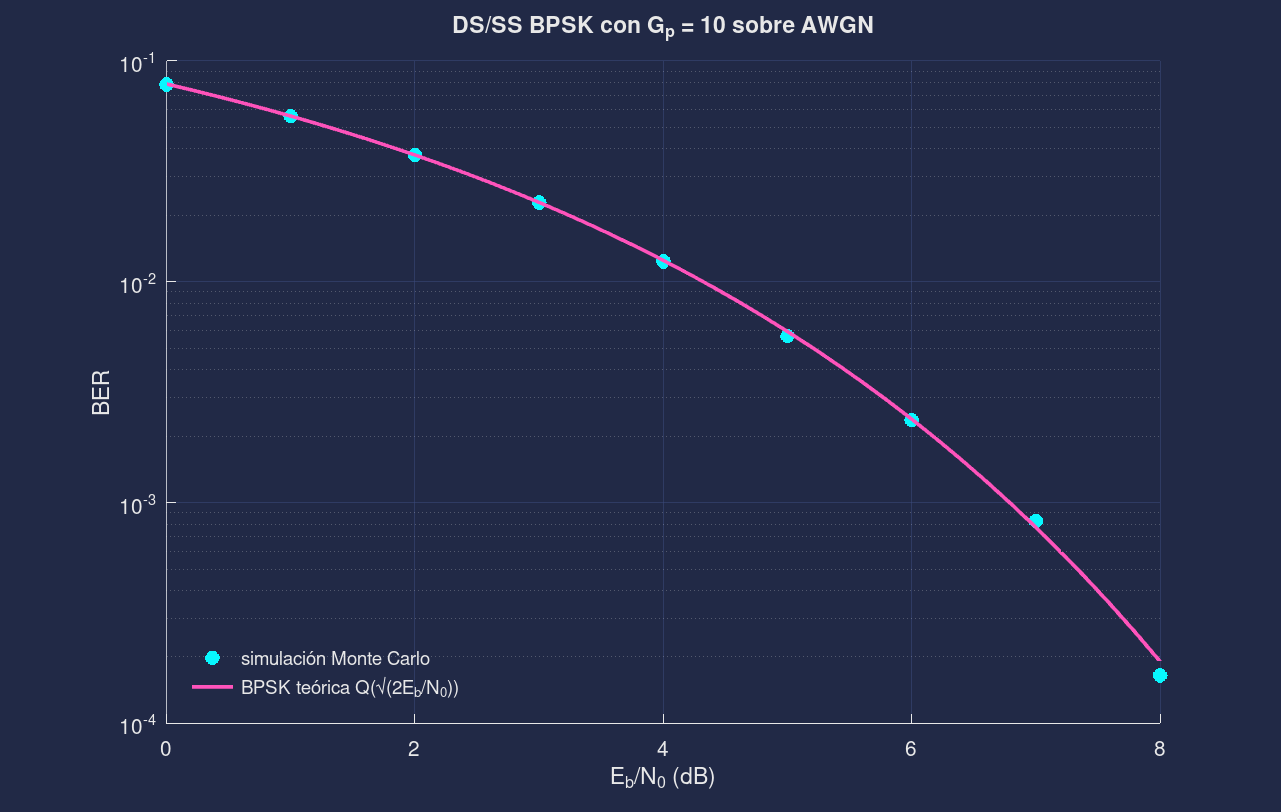
\includegraphics[width=0.9\linewidth]{p01_ber.png}
  \caption{BER de DS/SS BPSK con $G_p=10$ sobre AWGN, referida a $E_b/N_0$. La
  curva simulada se superpone a la de BPSK sin dispersión.}
  \label{fig:p01}
\end{figure}

\begin{table}[H]
  \centering
  \caption{BER medida y teórica para $G_p=10$ ($N=200\,000$ bits por punto).}
  \label{tab:p01}
  \begin{tabular}{@{}cccc@{}}
    \toprule
    $E_b/N_0$ (dB) & $P_e$ simulada & $P_e$ teórica & Error relativo \\
    \midrule
    0 & $7.82\times10^{-2}$ & $7.86\times10^{-2}$ & $-0.5\%$ \\
    1 & $5.62\times10^{-2}$ & $5.63\times10^{-2}$ & $-0.2\%$ \\
    2 & $3.75\times10^{-2}$ & $3.75\times10^{-2}$ & $+0.0\%$ \\
    3 & $2.28\times10^{-2}$ & $2.29\times10^{-2}$ & $-0.2\%$ \\
    4 & $1.24\times10^{-2}$ & $1.25\times10^{-2}$ & $-1.0\%$ \\
    5 & $5.68\times10^{-3}$ & $5.95\times10^{-3}$ & $-4.6\%$ \\
    6 & $2.37\times10^{-3}$ & $2.39\times10^{-3}$ & $-1.0\%$ \\
    7 & $8.25\times10^{-4}$ & $7.73\times10^{-4}$ & $+6.8\%$ \\
    8 & $1.65\times10^{-4}$ & $1.91\times10^{-4}$ & $-13.6\%$ \\
    \bottomrule
  \end{tabular}
\end{table}

\paragraph{Discusión.} El ensanchamiento del espectro no mejora la BER en un
canal AWGN: la señal dispersa ocupa $L$ veces más banda, pero también transmite
$L$ veces más chips por bit, y la energía por bit sigue siendo la misma. Dicho
de otro modo, el receptor desensancha la señal y queda con la misma
$E_b/N_0$ que tendría un sistema de banda angosta. La ventaja del espectro
disperso no está en la relación $E_b/N_0$, sino en la capacidad de rechazar
interferencia de banda angosta, en la baja probabilidad de interceptación
(problema 2) y en el acceso múltiple por código (problemas 7 y 8). El problema 3
muestra la misma simulación desde el otro punto de vista: referida al SNR de
entrada, la curva aparece desplazada 10 dB.

\paragraph{Código.}
\listado{problema01.m}

% ------------------------------------------------------------- problema 2
\section{Problema 2: detección de una señal LPI}

\begin{quote}
\itshape
Escriba un programa de MATLAB para realizar una simulación Monte Carlo de un
sistema de espectro disperso DS que opera en modo LPI. La ganancia de
procesamiento es 20 (13 dB) y la relación potencia de señal a ruido deseada es
$P_S/P_N$ en el receptor previo al desensanchamiento de la señal, 5 dB más
pequeña. Grafique la tasa de error medida como una función del SNR.
\end{quote}

\paragraph{Modelo.} Con $L=20$ chips por bit, $G_p=10\log_{10}20=13.01$ dB.
Antes de desensanchar, la señal está enterrada en el ruido:
$P_S/P_N=-5$ dB. Después del correlador, la ganancia de procesamiento se suma:
\begin{equation}
  \left.\frac{S}{N}\right|_\text{out}
  =\left.\frac{S}{N}\right|_\text{in}+G_p=-5+13.01=8.01\ \text{dB}
  \;\Longleftrightarrow\;
  \frac{E_b}{N_0}=10^{0.801}=6.32,
\end{equation}
y por tanto
\begin{equation}
  P_e=Q\!\left(\sqrt{2\times6.32}\right)=Q(3.55)\approx1.9\times10^{-4}.
\end{equation}

\paragraph{Método.} Se barrió el SNR de entrada entre $-20$ y $0$ dB con
$N=200\,000$ bits por punto, y se comparó con la curva teórica desplazada
13.01 dB. Para ilustrar el mecanismo LPI se generaron además 400 periodos del
código a $-5$ dB y se acumuló la correlación con el código correcto y con un
código desplazado un chip.

\paragraph{Resultados.} La figura~\ref{fig:p02ber} muestra que la BER medida
sigue a la teoría desplazada por $G_p$. En el punto de operación ($-5$ dB) se
midieron $1.95\times10^{-4}$ contra $1.88\times10^{-4}$ teóricos. La
figura~\ref{fig:p02t} muestra que, muestra a muestra, la señal es
indistinguible del ruido, pero el correlador la acumula de forma lineal mientras
el ruido crece como $\sqrt{n}$.

\begin{figure}[H]
  \centering
  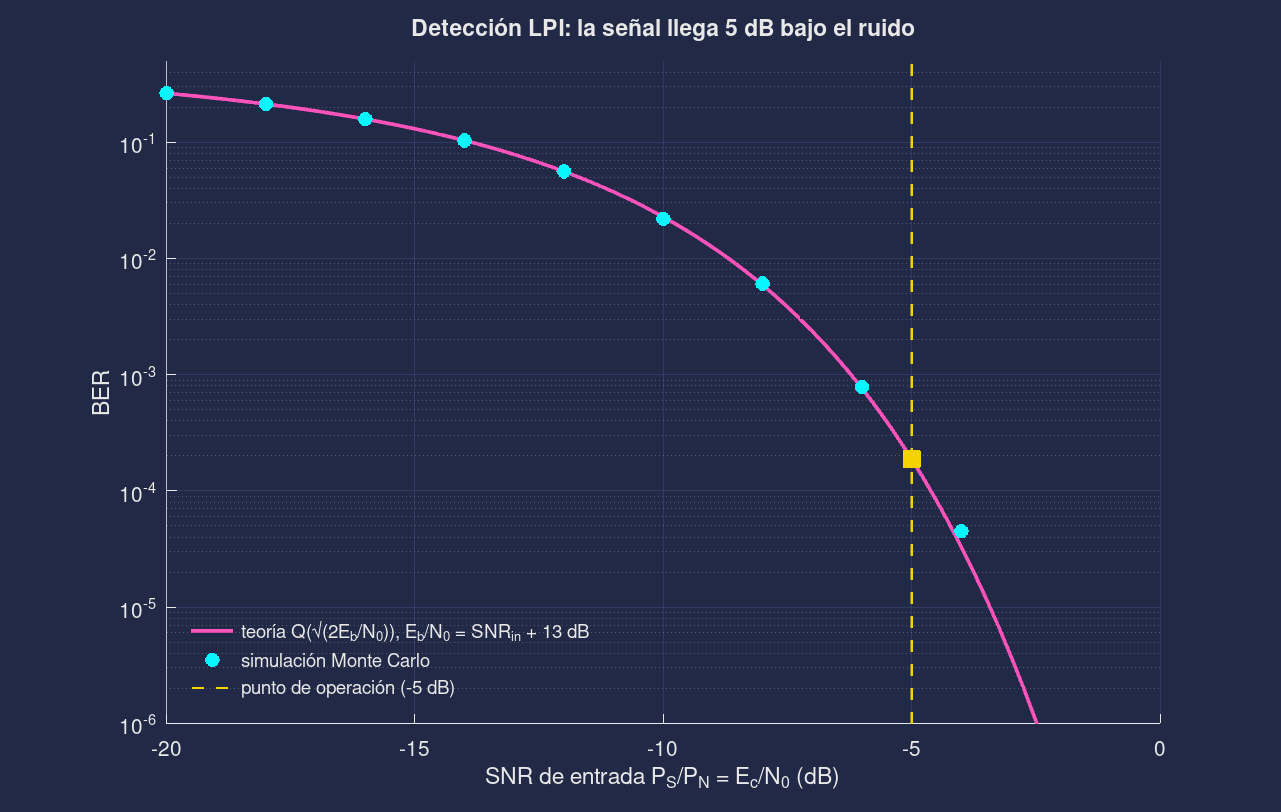
\includegraphics[width=0.9\linewidth]{p02_lpi_ber.png}
  \caption{BER contra el SNR de entrada para el sistema LPI. La curva de DS/SS
  está 13 dB a la izquierda de la de un receptor sin ganancia de procesamiento;
  el punto de operación es $-5$ dB.}
  \label{fig:p02ber}
\end{figure}

\begin{figure}[H]
  \centering
  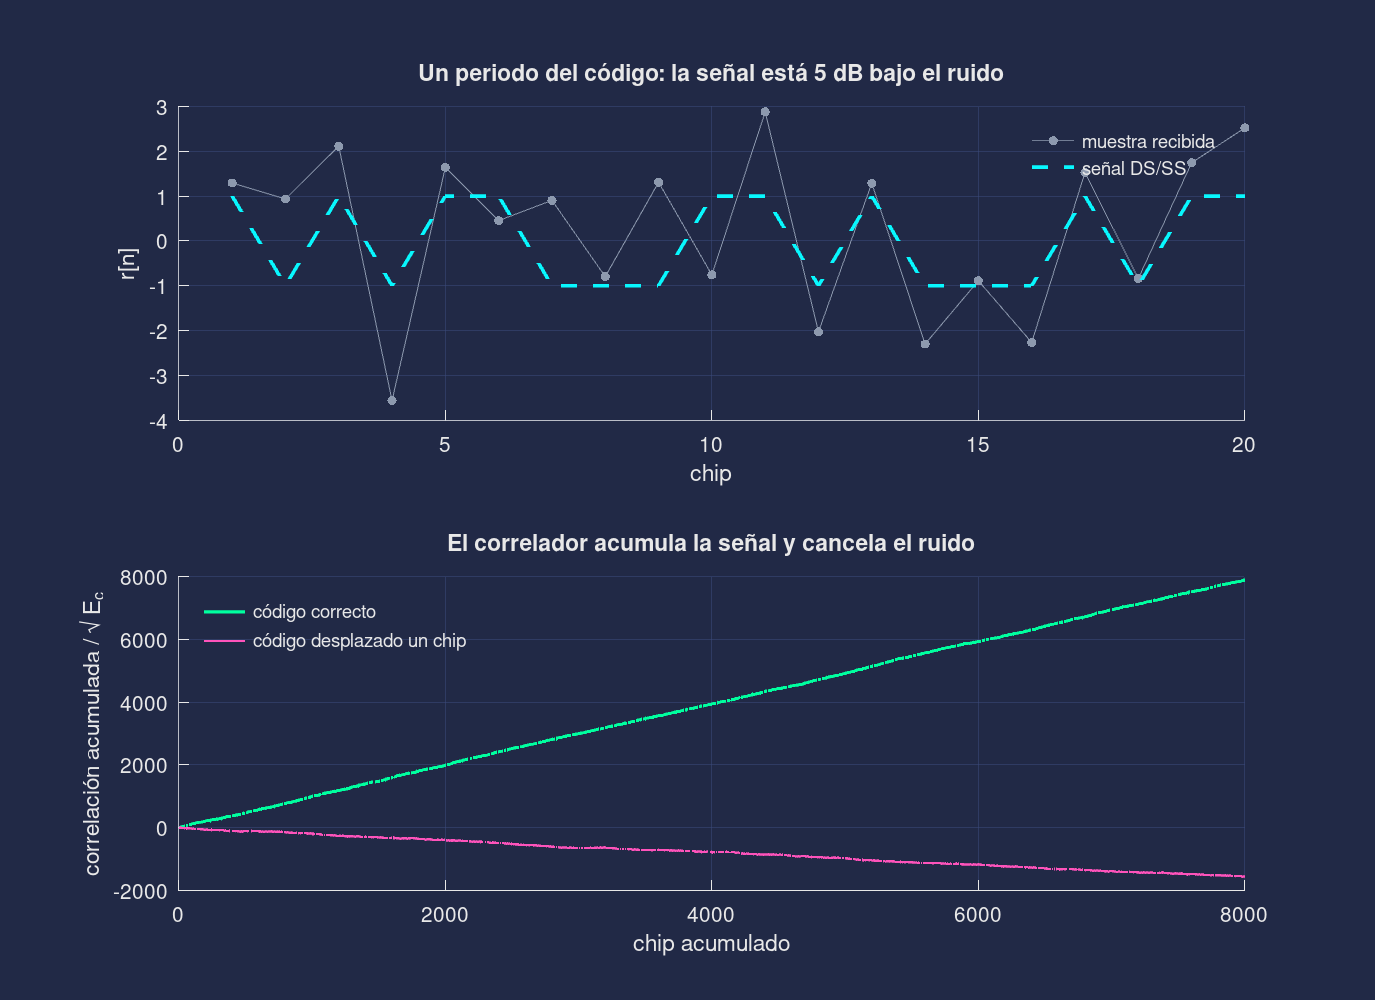
\includegraphics[width=0.92\linewidth]{p02_lpi_tiempo.png}
  \caption{Arriba: un periodo del código recibido a $-5$ dB; la señal (línea
  punteada) queda oculta bajo el ruido. Abajo: correlación acumulada durante 400
  periodos con el código correcto y con un código desplazado un chip.}
  \label{fig:p02t}
\end{figure}

\begin{table}[H]
  \centering
  \caption{BER del sistema LPI en función del SNR de entrada ($G_p=13.01$ dB).}
  \label{tab:p02}
  \begin{tabular}{@{}cccc@{}}
    \toprule
    $P_S/P_N$ (dB) & $P_e$ simulada & $P_e$ teórica & $E_b/N_0$ (dB) \\
    \midrule
    $-20$ & $2.64\times10^{-1}$ & $2.64\times10^{-1}$ & $-6.99$ \\
    $-16$ & $1.58\times10^{-1}$ & $1.58\times10^{-1}$ & $-2.99$ \\
    $-12$ & $5.61\times10^{-2}$ & $5.61\times10^{-2}$ & $1.01$ \\
    $-8$  & $6.08\times10^{-3}$ & $5.90\times10^{-3}$ & $5.01$ \\
    $-6$  & $7.85\times10^{-4}$ & $7.63\times10^{-4}$ & $7.01$ \\
    $-5$  & $1.95\times10^{-4}$ & $1.88\times10^{-4}$ & $8.01$ \\
    $-4$  & $4.50\times10^{-5}$ & $3.30\times10^{-5}$ & $9.01$ \\
    \bottomrule
  \end{tabular}
\end{table}

\paragraph{Discusión.} El sistema opera con una relación señal a ruido negativa
en la banda de transmisión y aun así alcanza una BER de $10^{-4}$: esa es la
esencia de una señal LPI. Un receptor que no conoce el código ve solo ruido; el
receptor legítimo, que puede reproducir la secuencia, gana $G_p$ dB al
correlacionar. La contraparte es que la interceptación es difícil pero no
imposible: un buscador de energía con un banco de correladores o un detector
cíclico puede encontrar la señal si la observa el tiempo suficiente, como
sugiere la rampa de la figura~\ref{fig:p02t}.

\paragraph{Código.}
\listado{problema02.m}

% ------------------------------------------------------------- problema 3
\section{Problema 3: ganancia de procesamiento con \texorpdfstring{$G_p=10$}{Gp=10}}

\begin{quote}
\itshape
Repita la simulación Monte Carlo descrita en el problema ilustrativo 4 para una
ganancia de procesamiento de 10 y grafique la tasa de error medida.
\end{quote}

\paragraph{Modelo.} Es el mismo sistema del problema 1, pero la abscisa es ahora
el SNR de entrada, es decir, la relación señal a ruido en la banda dispersa
($E_c/N_0$). La relación entre las dos referencias es
\begin{equation}
  \frac{E_b}{N_0}=\frac{E_c}{N_0}+10\log_{10}L
  =\frac{E_c}{N_0}+10\ \text{dB}.
\end{equation}
Por eso, si la BER se grafica contra $E_c/N_0$, la curva de DS/SS es la de BPSK
desplazada 10 dB hacia la izquierda: el receptor puede trabajar con 10 dB menos
de SNR en el canal para la misma BER. Esa es la ganancia de procesamiento.

\paragraph{Método.} Se simularon $N=200\,000$ bits por punto con $L=10$ chips,
barriendo $E_c/N_0$ de $-20$ a $-3$ dB, y se graficaron la curva medida, la
teoría de DS/SS referida a $E_c/N_0$ y la de BPSK referida a $E_b/N_0$.

\paragraph{Resultados.} La figura~\ref{fig:p03} muestra las dos curvas separadas
exactamente 10 dB. Por ejemplo, para $P_e\approx5\times10^{-2}$ BPSK necesita
$E_b/N_0\approx1.3$ dB, mientras que el sistema DS/SS lo consigue con
$E_c/N_0\approx-8.7$ dB.

\begin{figure}[H]
  \centering
  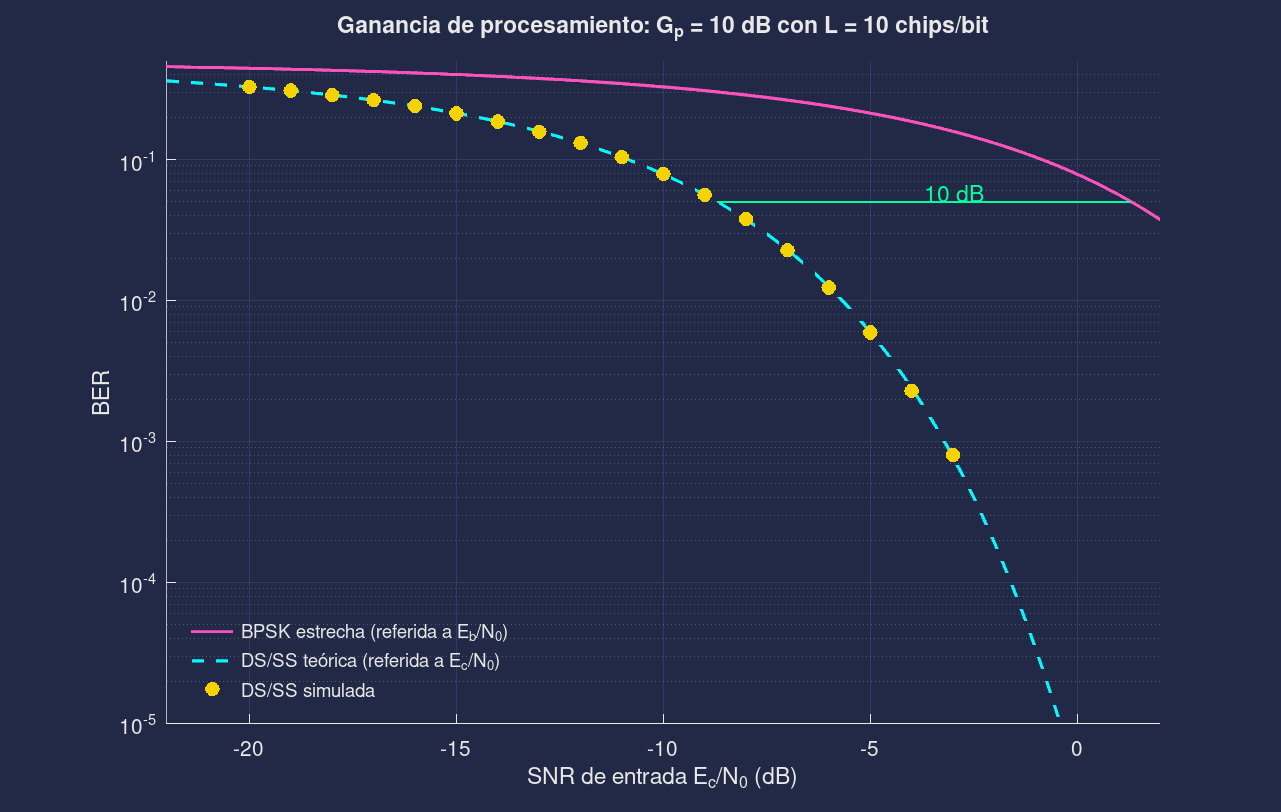
\includegraphics[width=0.9\linewidth]{p03_ganancia.png}
  \caption{BER contra el SNR de entrada. La curva de DS/SS (referida a
  $E_c/N_0$) está 10 dB a la izquierda de BPSK (referida a $E_b/N_0$): esa
  separación es la ganancia de procesamiento.}
  \label{fig:p03}
\end{figure}

\paragraph{Discusión.} Los problemas 1 y 3 dicen lo mismo desde dos ejes
distintos. Referida a $E_b/N_0$, la señal dispersa no gana nada; referida al SNR
del canal, gana exactamente $G_p$. La diferencia no es una contradicción: el
ensanchamiento compra 10 dB de margen contra el ruido del canal a cambio de
10 veces más banda. En un canal limitado por interferencia de banda angosta
(como en el problema 2) esa ganancia se convierte en rechazo de interferencia,
porque el receptor desensancha solo la porción de ruido que cae dentro de su
código.

\paragraph{Código.}
\listado{problema03.m}

% ------------------------------------------------------------- problema 4
\section{Problema 4: secuencia de longitud máxima con \texorpdfstring{$m=12$}{m=12}}

\begin{quote}
\itshape
Escriba un programa de MATLAB que implemente un registro de desplazamiento de
longitud máxima $m=12$ estados y genere cinco periodos de la secuencia. Calcule
y grafique la función de autocorrelación periódica de la secuencia bipolar
equivalente dada por (20).
\end{quote}

\paragraph{Modelo.} Se usó un LFSR de Fibonacci con el polinomio primitivo
\begin{equation}
  p(x)=x^{12}+x^6+x^4+1,
\end{equation}
cuya recurrencia es $s_{n+12}=s_{n+6}+s_{n+4}+s_n \pmod 2$. El periodo es
$L=2^{12}-1=4095$; el estado inicial $100\cdots0$ es no nulo, así que la
secuencia recorre todos los estados no nulos antes de repetirse. La
autocorrelación periódica de la secuencia bipolar se calculó con la
ecuación~\eqref{eq:autocorr} mediante la transformada de Fourier
($R=\mathrm{IFFT}(|X|^2)/L$), que es equivalente a la suma directa y mucho más
rápida para $L=4095$.

\paragraph{Resultados.} El script generó $5\times4095=20\,475$ chips y verificó
que los cinco periodos son idénticos. La secuencia tiene 2048 unos y 2047 ceros,
el balance exacto de una secuencia-$m$. La autocorrelación vale $R_c(0)=1$ y
$R_c(\tau)=-1/4095=-2.442\times10^{-4}$ para todo $\tau\neq0$, como muestra la
figura~\ref{fig:p04}: es una función de dos valores, con un pico 72.2 dB por
encima del lóbulo lateral.

\begin{figure}[H]
  \centering
  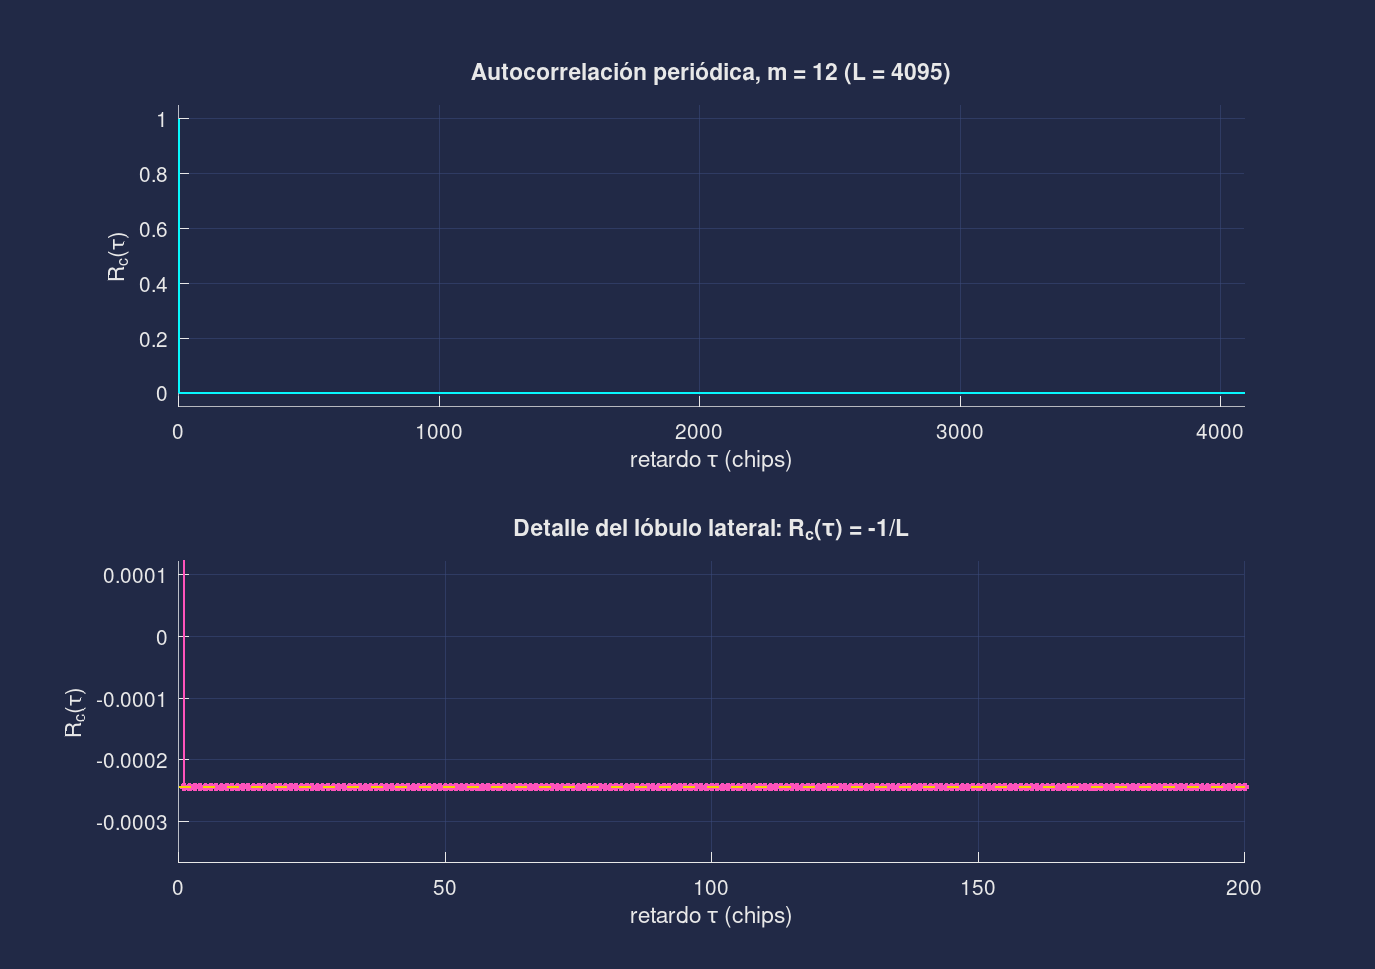
\includegraphics[width=0.92\linewidth]{p04_autocorrelacion.png}
  \caption{Autocorrelación periódica de la secuencia-$m$ de $m=12$. Arriba, el
  periodo completo; abajo, el detalle de los primeros retardos, donde se aprecia
  el lóbulo lateral constante en $-1/L$.}
  \label{fig:p04}
\end{figure}

\paragraph{Discusión.} La autocorrelación de dos valores es la propiedad que
hace útiles a las secuencias-$m$ para sincronización y para espectro disperso:
solo el retardo correcto produce un pico, y cualquier otro retardo da
prácticamente cero. Con $L=4095$ el lóbulo lateral es $1/4095$, es decir,
$-72$ dB, suficiente para que un correlador distinga el alineamiento correcto
aunque la señal esté muy por debajo del ruido.

\paragraph{Código.}
\listado{problema04.m}

% ------------------------------------------------------------- problema 5
\section{Problema 5: suma módulo 2 de dos secuencias-\texorpdfstring{$m$}{m}}

\begin{quote}
\itshape
Escriba un programa de MATLAB que implemente un registro de desplazamiento de
longitud máxima $m=3$ estados y $m=4$ estados y forme la suma módulo 2 de sus
secuencias de salida. ¿Es la secuencia resultante periódica? Si lo es, ¿cuál es
el periodo de la secuencia? Calcule y grafique la secuencia de autocorrelación
de la secuencia bipolar resultante utilizando (20).
\end{quote}

\paragraph{Modelo.} Se generaron las secuencias-$m$ de $m=3$
($p(x)=x^3+x+1$, $L=7$) y $m=4$ ($p(x)=x^4+x+1$, $L=15$). En bipolar, la suma
módulo 2 equivale al producto chip a chip:
\begin{equation}
  c_n = c_n^{(3)}\,c_n^{(4)}.
\end{equation}
Como ambas son periódicas, su producto también lo es, con periodo igual al
mínimo común múltiplo de los periodos:
\begin{equation}
  T=\operatorname{lcm}(7,15)=105.
\end{equation}

\paragraph{Resultados.} El periodo medido fue exactamente 105 chips: ningún
desplazamiento menor deja la secuencia igual. La figura~\ref{fig:p05} muestra la
secuencia compuesta y su autocorrelación. Los valores son
\begin{equation}
  R_c(\tau)=
  \begin{cases}
    1, & \tau\equiv0 \pmod{105},\\
    -1/15=-0.0667, & \tau\equiv0 \pmod 7,\ \tau\not\equiv0 \pmod{15},\\
    -1/7=-0.1429, & \tau\equiv0 \pmod{15},\ \tau\not\equiv0 \pmod 7,\\
    +1/105=0.0095, & \text{en otro caso}.
  \end{cases}
\end{equation}

\begin{figure}[H]
  \centering
  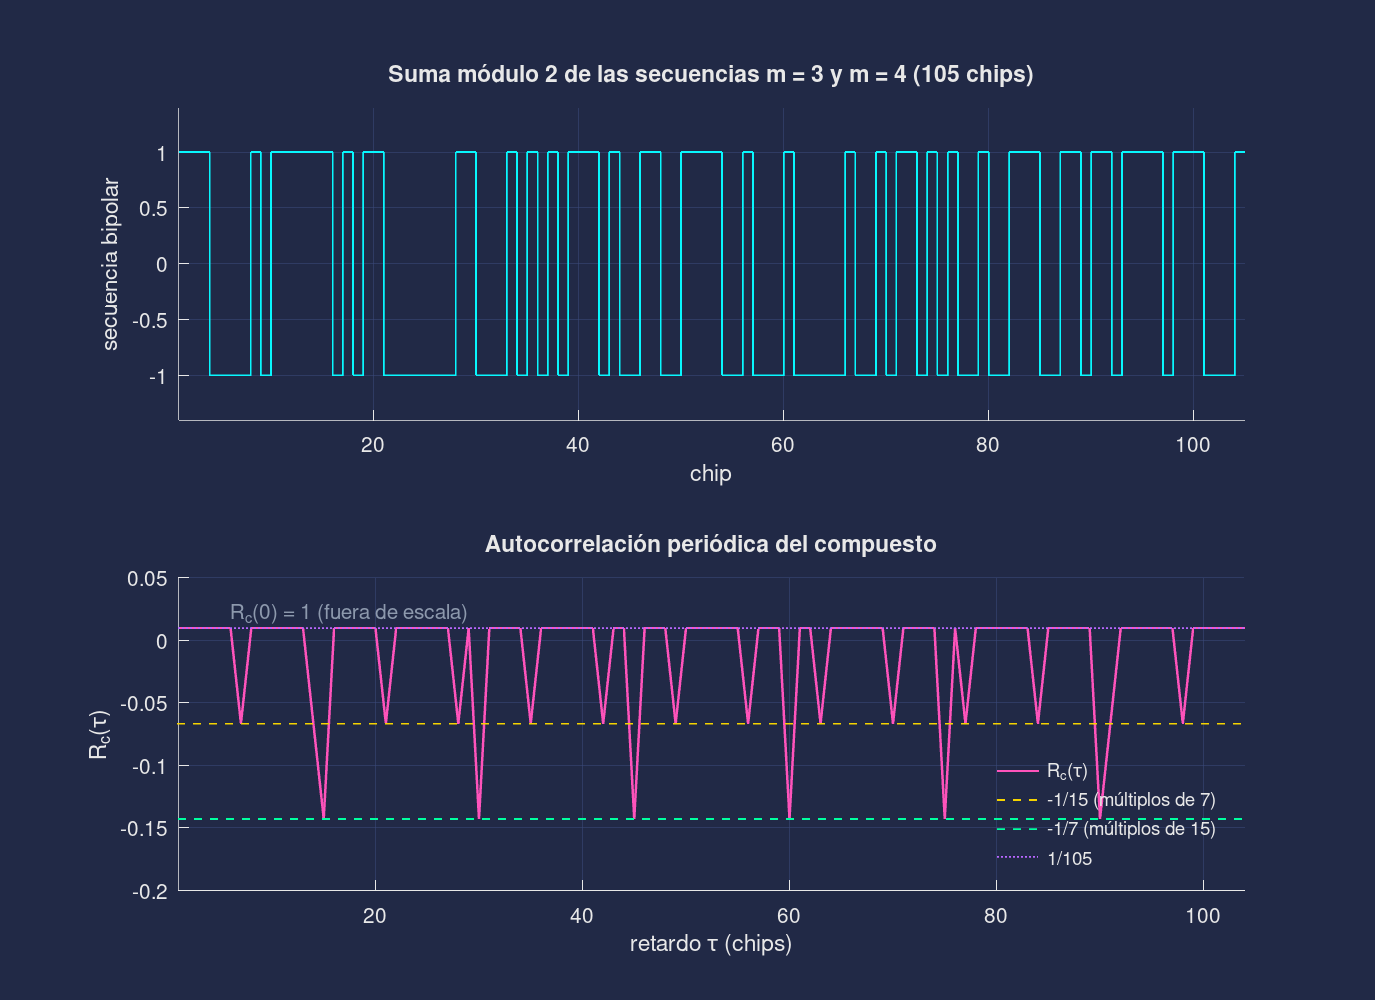
\includegraphics[width=0.92\linewidth]{p05_compuesta.png}
  \caption{Secuencia compuesta de 105 chips (arriba) y su autocorrelación
  periódica (abajo). Los mínimos en los múltiplos de 7 y de 15 son los lóbulos
  laterales grandes; $R_c(0)=1$ queda fuera de escala.}
  \label{fig:p05}
\end{figure}

\paragraph{Discusión.} La secuencia resultante es periódica, pero no es de
longitud máxima: su autocorrelación ya no es de dos valores y el peor lóbulo
lateral vale $-1/7$, es decir, solo 16.9 dB por debajo del pico. Como código de
espectro disperso es mucho peor que una secuencia-$m$ de 105 chips (que tendría
lóbulos de $-1/105$). Esto ilustra que combinar secuencias de periodos distintos
no produce una secuencia-$m$ más larga; para eso se necesitan polinomios
primitivos de grado mayor, o construcciones específicas como las secuencias Gold
del problema 6.

\paragraph{Código.}
\listado{problema05.m}

% ------------------------------------------------------------- problema 6
\section{Problema 6: autocorrelación de las secuencias Gold de \texorpdfstring{$L=31$}{L=31}}

\begin{quote}
\itshape
Escriba un programa de MATLAB para calcular la secuencia de autocorrelación de
las $L=31$ secuencias Gold que fueron generadas en el problema ilustrativo 6.
\end{quote}

\paragraph{Modelo.} Las secuencias Gold se construyen a partir de un par
preferido de secuencias-$m$ de la misma longitud. Se usó el par
\begin{equation}
  p_1(x)=x^5+x^2+1,\qquad p_2(x)=x^5+x^4+x^2+x+1,
\end{equation}
con $L=2^5-1=31$. Las 31 secuencias se obtienen como
\begin{equation}
  g_k(n)=a(n)\oplus b(n+k),\qquad k=0,\dots,30,
\end{equation}
donde $a$ y $b$ son las secuencias-$m$ bipolares. La autocorrelación de cada una
se calculó con la ecuación~\eqref{eq:autocorr}.

\paragraph{Resultados.} Las 31 autocorrelaciones toman solo tres valores en los
retardos distintos de cero,
\begin{equation}
  R_g(\tau)\in\left\{-\frac{9}{31},\ -\frac{1}{31},\ +\frac{7}{31}\right\}
  =\{-0.2903,\ -0.0323,\ +0.2258\},
\end{equation}
con las frecuencias que se muestran en la tabla~\ref{tab:p06}; en $\tau=0$ el
valor es 1. La correlación cruzada máxima de la familia es $9/31=0.2903$,
$-10.7$ dB respecto al pico.

\begin{table}[H]
  \centering
  \caption{Valores de la autocorrelación de las 31 secuencias Gold para
  $\tau\neq0$ (30 retardos por secuencia, 930 casos).}
  \label{tab:p06}
  \begin{tabular}{@{}cccc@{}}
    \toprule
    $31\,R_g(\tau)$ & $R_g(\tau)$ & Casos & Porcentaje \\
    \midrule
    $-9$ & $-0.2903$ & 180 & 19.4\% \\
    $-1$ & $-0.0323$ & 450 & 48.4\% \\
    $+7$ & $+0.2258$ & 300 & 32.3\% \\
    \bottomrule
  \end{tabular}
\end{table}

\begin{figure}[H]
  \centering
  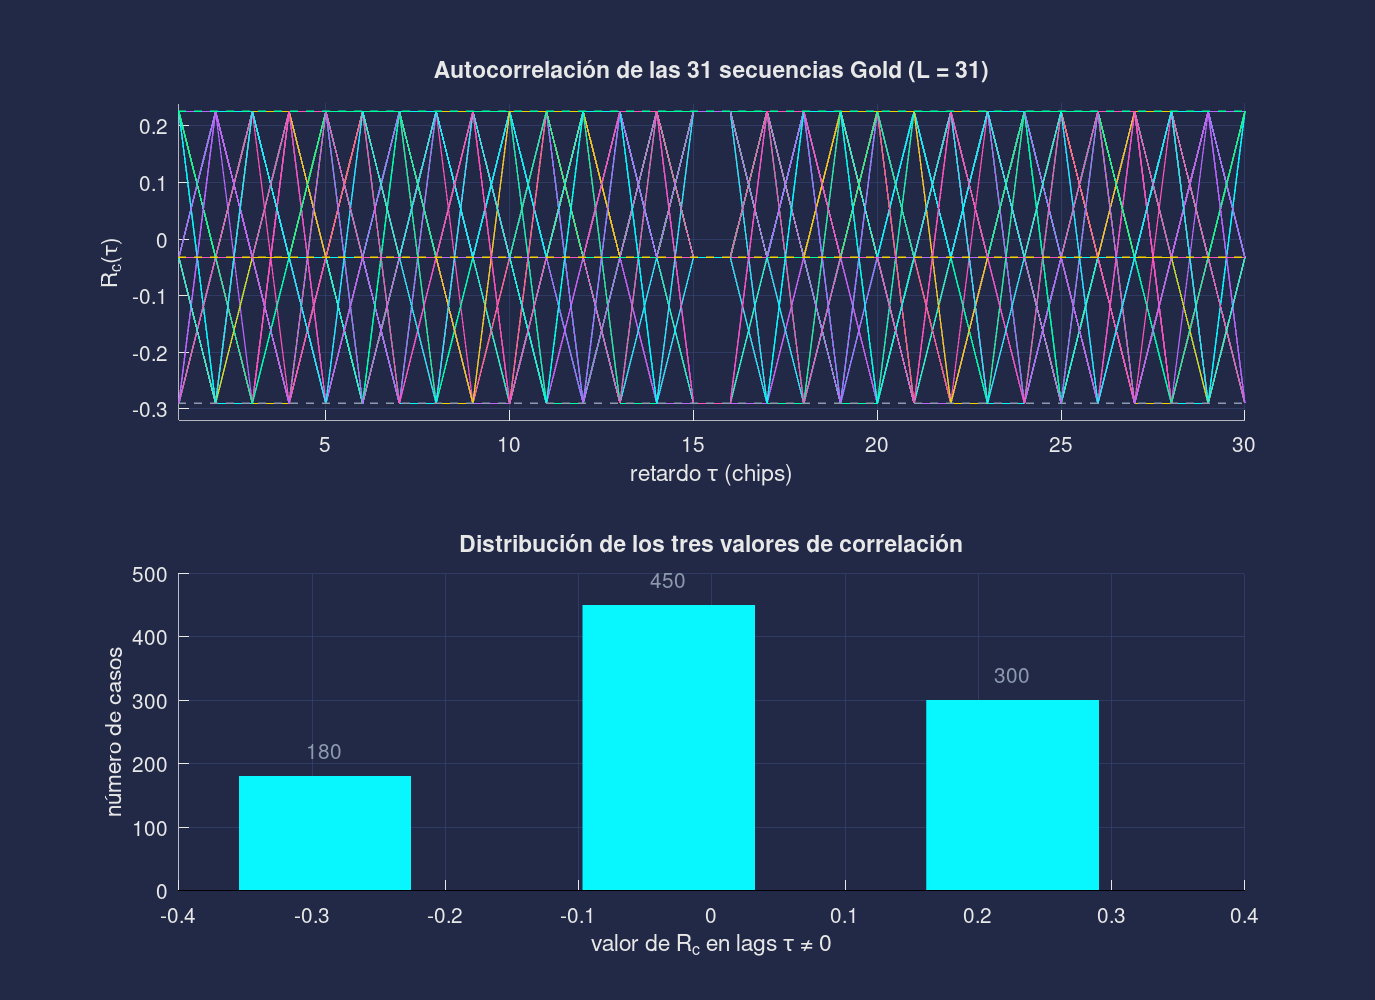
\includegraphics[width=0.92\linewidth]{p06_gold.png}
  \caption{Arriba: autocorrelación de las 31 secuencias Gold superpuestas; las
  líneas discontinuas marcan los tres niveles. Abajo: distribución de los tres
  valores.}
  \label{fig:p06}
\end{figure}

\paragraph{Discusión.} Las secuencias Gold sacrifican la autocorrelación ideal
de dos valores: sus lóbulos laterales llegan a $-0.29$, mucho peores que el
$-1/31=-0.032$ de una secuencia-$m$. A cambio, toda la familia comparte el mismo
conjunto pequeño de correlaciones cruzadas, lo que permite asignar un código
distinto a cada usuario y mantener la interferencia acotada. Es el compromiso
clásico en CDMA: se cambia autocorrelación por un conjunto grande de códigos con
correlación cruzada controlada. El mismo principio se usa en GPS, en los códigos
de aleatorización de WCDMA y en la sincronización de LTE.

\paragraph{Código.}
\listado{problema06.m}

% ------------------------------------------------------------- problema 7
\section{Problema 7: cuatro usuarios CDMA síncronos}

\begin{quote}
\itshape
Escriba un programa de MATLAB que realice una simulación Monte Carlo de cuatro
usuarios CDMA sincronizados en el tiempo cuando cada usuario emplea una secuencia
Gold distinta de longitud $L=31$. Las cuatro secuencias Gold pueden ser
seleccionadas de la tabla 3. Cada usuario emplea la modulación binaria $(\pm1)$
de su secuencia Gold representativa. El receptor para cada usuario correlaciona
la señal recibida CDMA compuesta, la cual es corrompida por ruido gaussiano
blanco aditivo (sumado en base a chip por chip) con cada secuencia respectiva al
usuario. Utilizando simulación Monte Carlo $N=10\,000$ bits de información,
estime y grafique la probabilidad de error para cada usuario como una función de
SNR.
\end{quote}

\paragraph{Modelo.} Cuatro usuarios transmiten con la misma amplitud por chip,
cada uno con su código Gold $c_k$ de 31 chips y datos $d_k(n)=\pm1$. La señal
recibida en el chip $i$ es
\begin{equation}
  r_i=\sum_{k=1}^{4}\sqrt{E_c}\,d_k(n)\,c_k(i)+w_i,
\end{equation}
con $w_i$ gaussiano de varianza $N_0/2$. El receptor del usuario $k$ correlaciona
su ventana de 31 chips con $c_k$ y decide por el signo. La interferencia de los
otros usuarios vale
\begin{equation}
  I_k=\sum_{j\neq k}\rho_{kj}\,d_j,\qquad
  \rho_{kj}=\frac{1}{31}\sum_{i=1}^{31} c_k(i)\,c_j(i).
\end{equation}
Para esta familia todos los $\rho_{kj}$ valen exactamente $-1/31$ en $\tau=0$,
así que la interferencia total de tres usuarios es
$3/31^2=0.0031$, es decir, 25.1 dB por debajo de la señal.

\paragraph{Método.} Se simularon $N=10\,000$ bits por usuario para
$E_b/N_0=0,\dots,9$ dB, con $E_c=1$ y $E_b=31$. El motor
(\texttt{comun/simular\_cdma.m}) genera la señal compuesta chip por chip, suma el
ruido y desensancha cada usuario con su propio código.

\paragraph{Resultados.} La figura~\ref{fig:p07} y la tabla~\ref{tab:p07}
muestran que los cuatro usuarios siguen la curva de un usuario aislado. La
diferencia es despreciable hasta 9 dB, donde la interferencia residual empieza a
notarse en el cuarto decimal.

\begin{figure}[H]
  \centering
  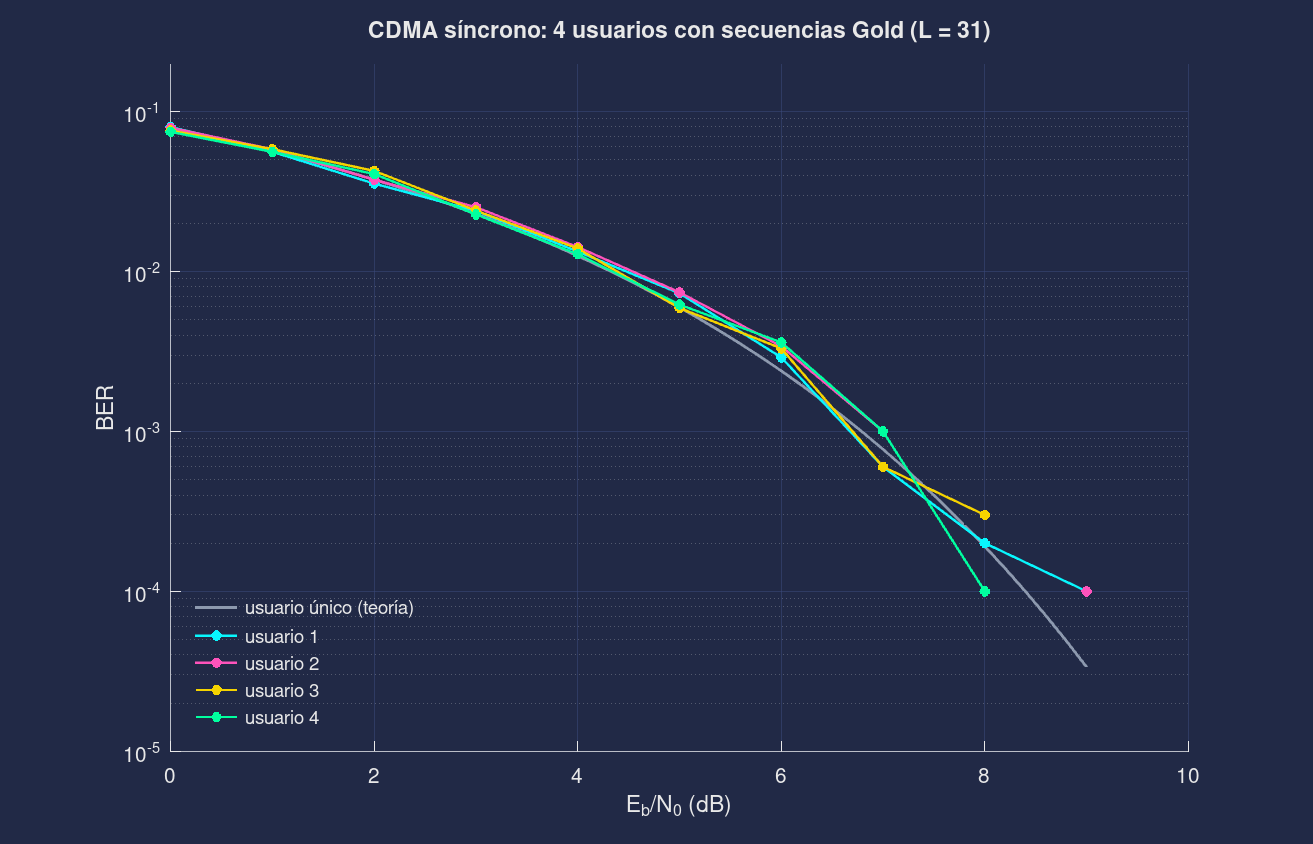
\includegraphics[width=0.9\linewidth]{p07_cdma_sincrono.png}
  \caption{CDMA síncrono con cuatro usuarios y secuencias Gold de 31 chips. Las
  cuatro curvas se superponen a la teoría de un usuario aislado.}
  \label{fig:p07}
\end{figure}

\begin{table}[H]
  \centering
  \caption{BER por usuario en el sistema CDMA síncrono ($N=10\,000$ bits).}
  \label{tab:p07}
  \begin{tabular}{@{}cccccc@{}}
    \toprule
    $E_b/N_0$ (dB) & Usuario 1 & Usuario 2 & Usuario 3 & Usuario 4 & Teoría \\
    \midrule
    0 & $7.99\times10^{-2}$ & $7.91\times10^{-2}$ & $7.59\times10^{-2}$ & $7.45\times10^{-2}$ & $7.86\times10^{-2}$ \\
    3 & $2.39\times10^{-2}$ & $2.52\times10^{-2}$ & $2.40\times10^{-2}$ & $2.27\times10^{-2}$ & $2.29\times10^{-2}$ \\
    6 & $2.90\times10^{-3}$ & $3.40\times10^{-3}$ & $3.30\times10^{-3}$ & $3.60\times10^{-3}$ & $2.39\times10^{-3}$ \\
    9 & $1.00\times10^{-4}$ & $1.00\times10^{-4}$ & $0$ & $0$ & $3.36\times10^{-5}$ \\
    \bottomrule
  \end{tabular}
\end{table}

\paragraph{Discusión.} Aunque las secuencias Gold no son ortogonales, en el
enlace síncrono todas las correlaciones cruzadas a retardo cero valen $-1/31$,
de modo que la interferencia múltiple es 25 dB menor que la señal. Para un
sistema con $E_b/N_0$ de interés práctico (hasta 10--12 dB) el CDMA síncrono se
comporta como un sistema de un solo usuario. El piso de interferencia aparece
alrededor de $E_b/N_0\approx25$ dB, fuera del rango útil. Esto explica por qué el
enlace descendente (síncrono) es más benigno que el ascendente (asíncrono), que
se estudia en el problema 8.

\paragraph{Código.}
\listado{problema07.m}

% ------------------------------------------------------------- problema 8
\section{Problema 8: los mismos usuarios, ahora asíncronos}

\begin{quote}
\itshape
Repita el problema 7 cuando los cuatro usuarios transmiten asíncronamente. Por
ejemplo, simule el caso cuando las cuatro señales CDMA utilizadas estén
desfasadas en tiempo por un chip en relación con las otras señales. Esto es, la
señal CDMA del usuario 2 es retrasada por un chip en relación al primer usuario,
la señal CDMA del usuario 3 es retrasada por un chip en relación a la señal del
usuario 2 y la señal CDMA del usuario 4 es retrasada por un chip en relación a la
señal del usuario 3. Compare la probabilidad de error obtenida con transmisión
asíncrona con la obtenida con transmisión síncrona.
\end{quote}

\paragraph{Modelo.} Es el mismo sistema, con retardos $[0,1,2,3]$ chips. Cada
receptor sigue sincronizado con su propio usuario: desensancha la ventana que
empieza en su retardo. Como los bits de los interferentes ya no están alineados
con esa ventana, la interferencia deja de ser la correlación de periodo completo
y se convierte en una correlación parcial, que puede alcanzar $9/31$ en lugar de
$1/31$. La interferencia deja de estar 25 dB abajo y pasa a estar alrededor de
10 dB abajo, suficiente para crear un piso de error.

\paragraph{Método.} Se corrió el mismo motor con retardos $[0,1,2,3]$ y con
retardos nulos, para $N=10\,000$ bits y $E_b/N_0=0,\dots,9$ dB.

\paragraph{Resultados.} La figura~\ref{fig:p08} compara las dos situaciones y la
tabla~\ref{tab:p08} resume los valores. A 9 dB, el promedio síncrono es
$1.0\times10^{-4}$ y el asíncrono $4.2\times10^{-3}$, 42 veces mayor. Los pisos
dependen del usuario: el usuario 2 (retardo de un chip) termina en
$5\times10^{-4}$, mientras que los usuarios 1 y 3 quedan alrededor de
$6.7\times10^{-3}$.

\begin{figure}[H]
  \centering
  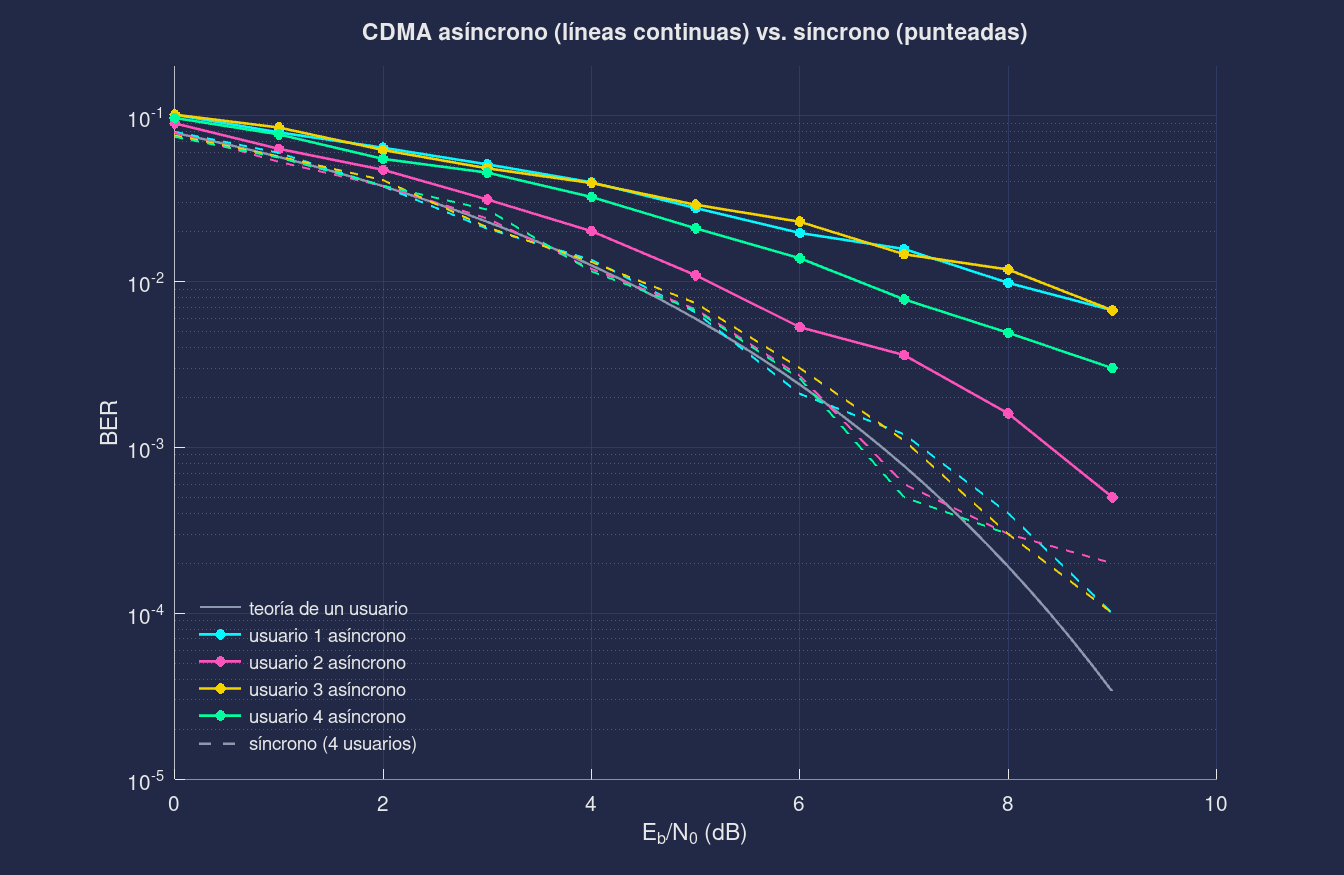
\includegraphics[width=0.92\linewidth]{p08_cdma_asincrono.png}
  \caption{CDMA asíncrono (líneas continuas con marcadores) contra síncrono
  (líneas punteadas). El desfase de un chip entre usuarios elimina la
  ortogonalidad y produce un piso de BER.}
  \label{fig:p08}
\end{figure}

\begin{table}[H]
  \centering
  \caption{BER con transmisión síncrona (promedio de los cuatro usuarios) y
  asíncrona (por usuario) para los mismos códigos y retardos.}
  \label{tab:p08}
  \begin{tabular}{@{}cccccc@{}}
    \toprule
    $E_b/N_0$ (dB) & Síncrono (media) & Asíncrono u1 & u2 & u3 & u4 \\
    \midrule
    0 & $7.7\times10^{-2}$ & $1.01\times10^{-1}$ & $8.98\times10^{-2}$ & $1.01\times10^{-1}$ & $9.68\times10^{-2}$ \\
    3 & $2.3\times10^{-2}$ & $5.08\times10^{-2}$ & $3.12\times10^{-2}$ & $4.81\times10^{-2}$ & $4.53\times10^{-2}$ \\
    6 & $2.6\times10^{-3}$ & $1.96\times10^{-2}$ & $5.30\times10^{-3}$ & $2.29\times10^{-2}$ & $1.38\times10^{-2}$ \\
    9 & $1.0\times10^{-4}$ & $6.70\times10^{-3}$ & $5.00\times10^{-4}$ & $6.70\times10^{-3}$ & $3.00\times10^{-3}$ \\
    \bottomrule
  \end{tabular}
\end{table}

\paragraph{Discusión.} El asincronismo destruye la propiedad que hacía ortogonal
al CDMA síncrono: las correlaciones parciales ya no se cancelan y la
interferencia múltiple se convierte en el límite dominante. Por eso los sistemas
celulares reales usan el enlace descendente con códigos ortogonales y
sincronización de trama, mientras que el enlace ascendente requiere control de
potencia, códigos más largos y, en la práctica, receptores multiusuario. La
diferencia entre usuarios (el usuario 2 tiene un piso 13 veces menor que el 1)
muestra que el desempeño asíncrono depende de la combinación particular de
retardos, no solo del número de usuarios.

\paragraph{Código.}
\listado{problema08.m}

% ------------------------------------------------------------- problema 9
\section{Problema 9: patrón de salto de frecuencia con \texorpdfstring{$m=7$}{m=7}}

\begin{quote}
\itshape
Un sistema FSK ortogonal binario FH emplea un registro de desplazamiento de
$m=7$ estados para generar una secuencia de longitud máxima periódica de longitud
$L=127$. Cada estado del registro de desplazamiento selecciona una de $N=127$
bandas de frecuencia que no se traslapan en el patrón de salto. Escriba un
programa de MATLAB que simule la selección de la frecuencia central y la
generación de dos frecuencias en cada una de las $N=127$ bandas de frecuencia.
Demuestre el patrón de selección de frecuencia para los primeros 10 intervalos
de bit.
\end{quote}

\paragraph{Modelo.} El registro de 7 etapas usa el polinomio primitivo
$p(x)=x^7+x^3+1$ y recorre los 127 estados no nulos. El estado binario se
interpreta como un entero entre 0 y 127 y se mapea a la banda
\begin{equation}
  b_n=\operatorname{dec}(s_{n-1}\cdots s_{n-7})+1\in\{1,\dots,127\}.
\end{equation}
Como el registro pasa por todos los estados no nulos, el patrón es una
permutación de las 127 bandas: ninguna se repite antes de agotar el periodo.
Cada banda ocupa $\Delta f$ y contiene dos tonos FSK en
$f_n\pm\Delta f/4$; con $\Delta f=25$ kHz, los tonos quedan separados 12.5 kHz,
que es $1/T_b$ para $T_b=80\,\mu$s, la separación necesaria para detección no
coherente ortogonal.

\paragraph{Método.} Se calentó el registro 40 saltos para evitar que los primeros
estados sean solo corrimientos del estado inicial, y se registraron los
siguientes 10 intervalos de bit. Para cada banda se calcularon el centro y los
dos tonos.

\paragraph{Resultados.} La secuencia de bandas de los primeros 10 bits es
\begin{equation}
  60,\ 120,\ 112,\ 95,\ 61,\ 122,\ 115,\ 102,\ 76,\ 23.
\end{equation}
La figura~\ref{fig:p09} muestra el patrón, el salto en frecuencia y el detalle de
la banda 60 con sus dos tonos. La tabla~\ref{tab:p09} lista los estados y las
frecuencias.

\begin{table}[H]
  \centering
  \caption{Patrón de selección de frecuencia para los primeros 10 intervalos.}
  \label{tab:p09}
  \begin{tabular}{@{}cccccc@{}}
    \toprule
    Bit & Estado & Banda & Centro (MHz) & Tono 1 (MHz) & Tono 2 (MHz) \\
    \midrule
    1 & 0111011 & 60  & 901.475 & 901.46875 & 901.48125 \\
    2 & 1110111 & 120 & 902.975 & 902.96875 & 902.98125 \\
    3 & 1101111 & 112 & 902.775 & 902.76875 & 902.78125 \\
    4 & 1011110 & 95  & 902.350 & 902.34375 & 902.35625 \\
    5 & 0111100 & 61  & 901.500 & 901.49375 & 901.50625 \\
    6 & 1111001 & 122 & 903.025 & 903.01875 & 903.03125 \\
    7 & 1110010 & 115 & 902.850 & 902.84375 & 902.85625 \\
    8 & 1100101 & 102 & 902.525 & 902.51875 & 902.53125 \\
    9 & 1001011 & 76  & 901.875 & 901.86875 & 901.88125 \\
    10 & 0010110 & 23 & 900.550 & 900.54375 & 900.55625 \\
    \bottomrule
  \end{tabular}
\end{table}

\begin{figure}[H]
  \centering
  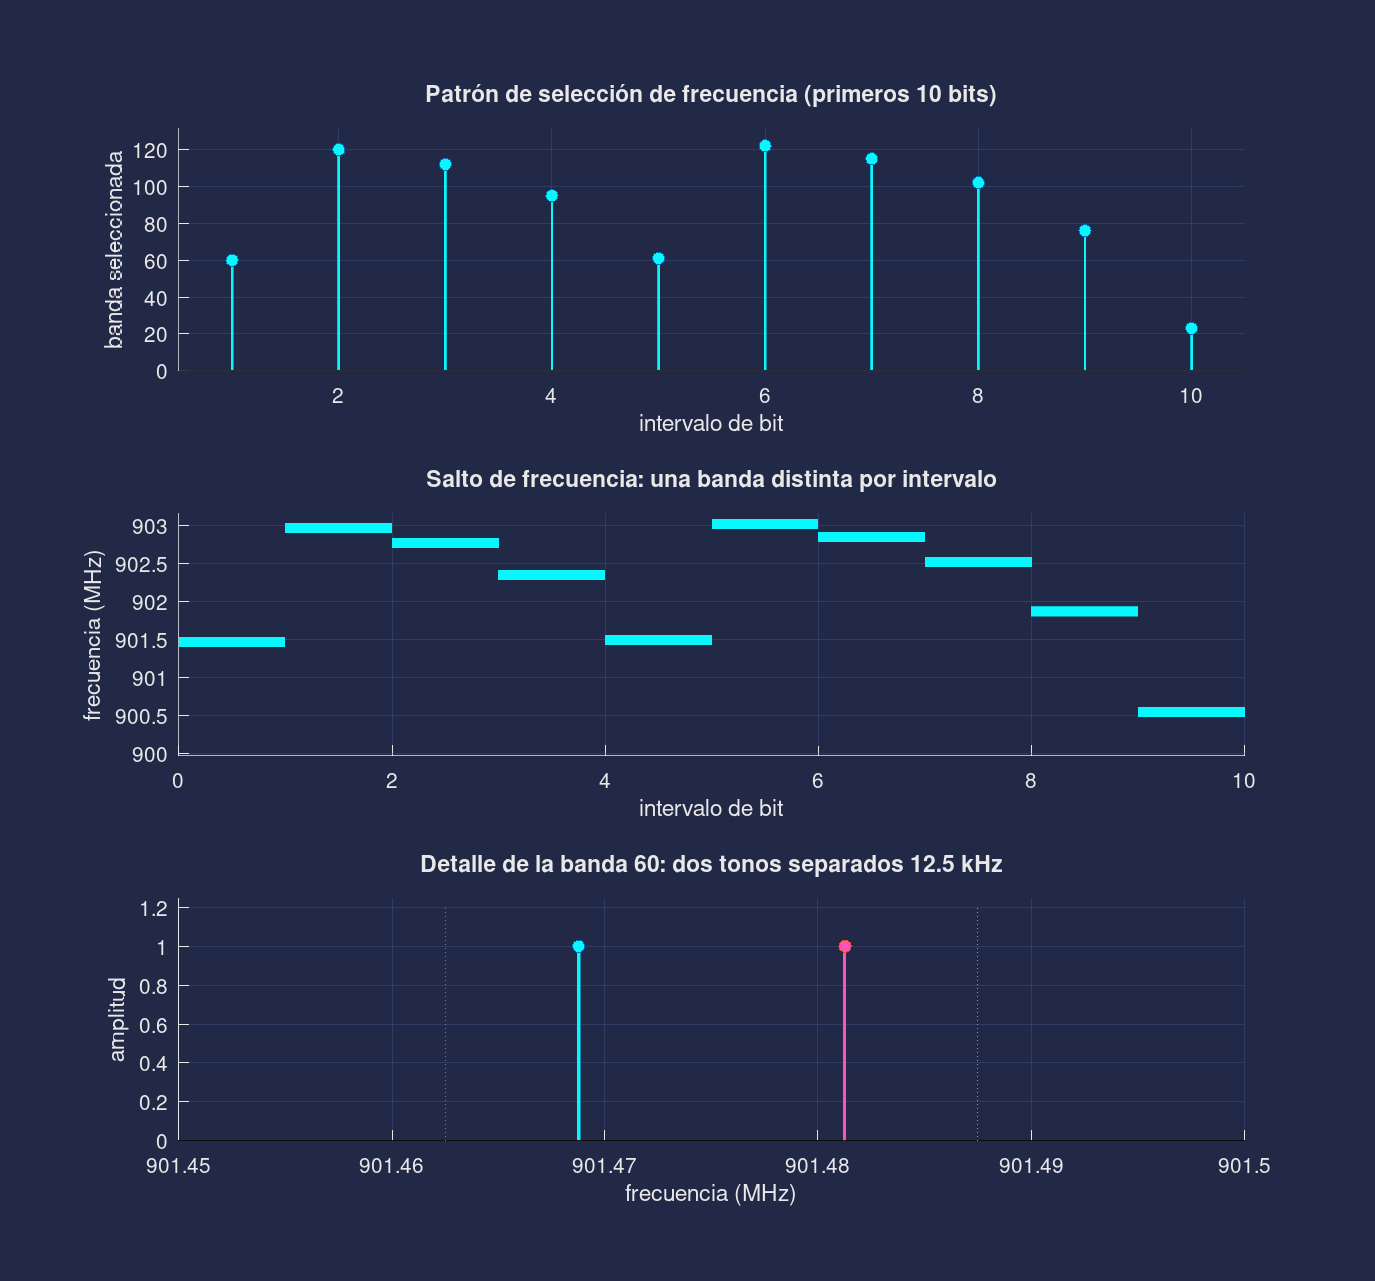
\includegraphics[width=0.9\linewidth]{p09_fh_patron.png}
  \caption{Patrón de salto: banda seleccionada por intervalo (arriba), salto en
  frecuencia (centro) y detalle de los dos tonos FSK de la banda 60 (abajo), con
  las fronteras de la banda en líneas punteadas.}
  \label{fig:p09}
\end{figure}

\paragraph{Discusión.} El registro de desplazamiento es a la vez el generador de
la secuencia pseudoaleatoria y el seleccionador de banda: los 127 estados son
las 127 bandas. El patrón es determinístico y reproducible por el receptor, pero
para un observador externo parece aleatorio. Los dos tonos dentro de cada banda
permiten transmitir un bit FSK por salto; como las bandas no se traslapan y los
tonos están separados $1/T_b$, la detección no coherente es ortogonal y la
probabilidad de error por salto es $P_e=\tfrac12 e^{-E_b/2N_0}$.

\paragraph{Código.}
\listado{problema09.m}

% ------------------------------------------------------------- problema 10
\section{Problema 10: FH/FSK con interferencia de banda parcial}

\begin{quote}
\itshape
Escriba un programa Monte Carlo para simular un sistema de comunicación digital
FH que emplee FSK binario con detección no coherente (ley cuadrada). El sistema
es corrompido por interferencia de banda parcial con densidad espectral $J_0/\alpha$,
donde $\alpha=0.1$. La interferencia es espectralmente plana sobre la banda de
frecuencia $0<\alpha\le0.1$. Grafique la tasa de error medida para este sistema
vs el SNR $E_b/J_0$.
\end{quote}

\paragraph{Modelo.} En cada salto, con probabilidad $\alpha$ la señal cae en la
subbanda interferida; en ese caso la densidad de interferencia es $J_0/\alpha$
(y cero fuera de ella). Con detección no coherente de ley cuadrática y ruido
térmico despreciable,
\begin{equation}
  P_e(\text{sin interferencia})=0,\qquad
  P_e(\text{interferido})=\frac12\exp\!\left(-\frac{E_b}{2J_0/\alpha}\right),
\end{equation}
de modo que
\begin{equation}
  P_e=(1-\alpha)\cdot0+\alpha\cdot\frac12
  \exp\!\left(-\frac{\alpha E_b}{2J_0}\right)
  =\frac{\alpha}{2}\exp\!\left(-\frac{\alpha E_b}{2J_0}\right).
\end{equation}

\paragraph{Método.} Para cada $E_b/J_0$ se simularon $N=500\,000$ bits con
$J_0=1$ y $N_0=0$. En cada bit se sortea si el salto cae en la banda interferida
y se generan dos muestras complejas de ruido con varianza $J_0/\alpha$; se
comparan las energías de los dos tonos.

\paragraph{Resultados.} La figura~\ref{fig:p10} y la tabla~\ref{tab:p10}
muestran que la simulación sigue la teoría. A 20 dB, la BER medida es
$3.86\times10^{-4}$ frente a $3.37\times10^{-4}$ teórica. La curva de banda
completa ($\alpha=1$) se incluye como referencia: a 10 dB ya está en
$3.4\times10^{-3}$ y a 20 dB es del orden de $10^{-22}$, mientras que la
interferencia parcial mantiene la BER en $10^{-4}$.

\begin{figure}[H]
  \centering
  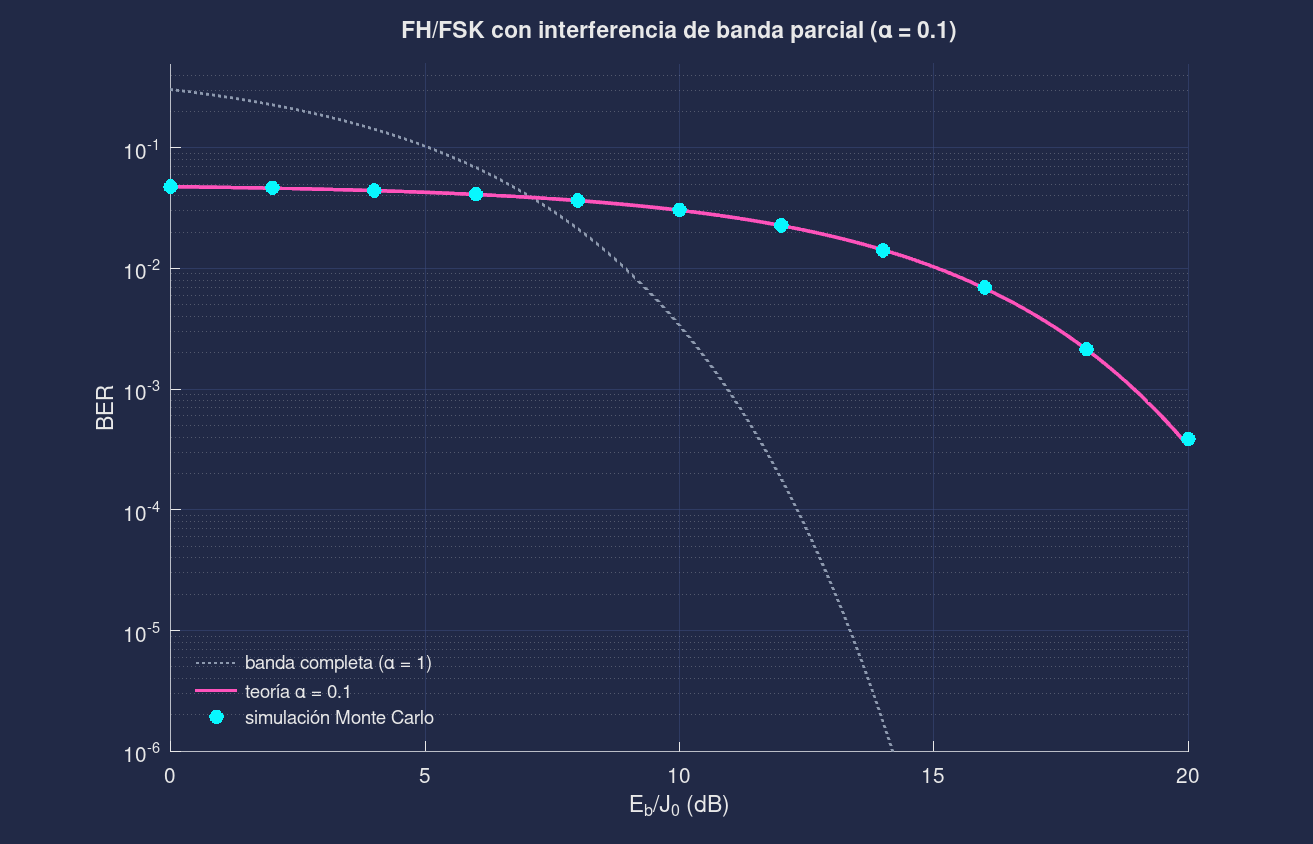
\includegraphics[width=0.9\linewidth]{p10_fh_banda_parcial.png}
  \caption{FH/FSK con interferencia de banda parcial ($\alpha=0.1$). La curva
  punteada es la referencia de un interferidor de banda completa.}
  \label{fig:p10}
\end{figure}

\begin{table}[H]
  \centering
  \caption{BER del FH/FSK con $\alpha=0.1$ ($N=500\,000$ bits).}
  \label{tab:p10}
  \begin{tabular}{@{}ccc@{}}
    \toprule
    $E_b/J_0$ (dB) & $P_e$ simulada & $P_e$ teórica \\
    \midrule
    0  & $4.76\times10^{-2}$ & $4.76\times10^{-2}$ \\
    6  & $4.12\times10^{-2}$ & $4.10\times10^{-2}$ \\
    12 & $2.27\times10^{-2}$ & $2.26\times10^{-2}$ \\
    16 & $6.95\times10^{-3}$ & $6.83\times10^{-3}$ \\
    20 & $3.86\times10^{-4}$ & $3.37\times10^{-4}$ \\
    \bottomrule
  \end{tabular}
\end{table}

\paragraph{Discusión.} La interferencia de banda parcial es mucho más dañina que
la de banda completa: el interferidor concentra su potencia en el 10\% de la
banda, de modo que cuando el salto cae ahí la relación señal a interferencia se
degrada en un factor $1/\alpha=10$. La BER decae exponencialmente, no como una
función $Q$: para reducirla en un factor $e$ hay que aumentar $E_b/J_0$ en
$2/\alpha=20$ unidades, es decir, 13 dB. Por eso un interferidor inteligente
elige $\alpha$ para maximizar la BER, y el diseño FH debe combinarse con
codificación, entrelazado o saltos más rápidos para que la interferencia se
promedie.

\paragraph{Código.}
\listado{problema10.m}

% ------------------------------------------------------------- problema 11
\section{Problema 11: diversidad dual con pesos adaptativos}

\begin{quote}
\itshape
Repita la simulación Monte Carlo en el problema ilustrativo 8 cuando el peso
utilizado en el combinador en la ausencia de interferencia es fijo a $w=50$ y con
interferencia el peso es $w=1/\sigma^2=2/E$, donde la energía de la señal es
$E\ge4$. Grafique la tasa de error medida a partir de la simulación Monte Carlo
para este sistema de diversidad dual y compare este desempeño con el obtenido en
el problema ilustrativo 8.
\end{quote}

\paragraph{Modelo.} Cada bit se transmite en dos saltos independientes; cada
salto se interfiere con probabilidad $\alpha=0.1$. El receptor combina las
salidas de ley cuadrática de los dos saltos con pesos $w_1,w_2$:
\begin{equation}
  \Lambda=w_1\left(|r_{1,1}|^2-|r_{2,1}|^2\right)
         +w_2\left(|r_{1,2}|^2-|r_{2,2}|^2\right),
\end{equation}
y decide por el signo. En el ejemplo ilustrativo los dos pesos son iguales
($w_1=w_2=1$). En este problema el receptor tiene información del estado de cada
salto y usa
\begin{equation}
  w=\begin{cases}
    50, & \text{salto sin interferencia},\\[2pt]
    \dfrac{1}{\sigma^2}=\dfrac{2}{E}, & \text{salto interferido},\ E\ge4.
  \end{cases}
\end{equation}
El valor 50 es una escala fija; lo que importa es la relación con $2/E$, que
hace que el salto interferido pese cada vez menos a medida que crece la energía.

\paragraph{Método.} Se simularon $N=500\,000$ bits para $E=7,\dots,17$ dB
($E\ge5>4$), con $J_0=1$, $N_0=0$ y dos saltos por bit. Se compararon el
combinador de pesos iguales y el ponderado.

\paragraph{Resultados.} La figura~\ref{fig:p11} y la tabla~\ref{tab:p11}
muestran la mejora. A 7 dB, el combinador de pesos iguales da
$4.55\times10^{-2}$ y el ponderado $3.18\times10^{-3}$: 14 veces menos errores.
La ventaja disminuye al aumentar $E$ (2.9 veces a 15 dB) y se reduce a
1.5 veces a 17 dB, donde el salto interferido ya no domina.

\begin{figure}[H]
  \centering
  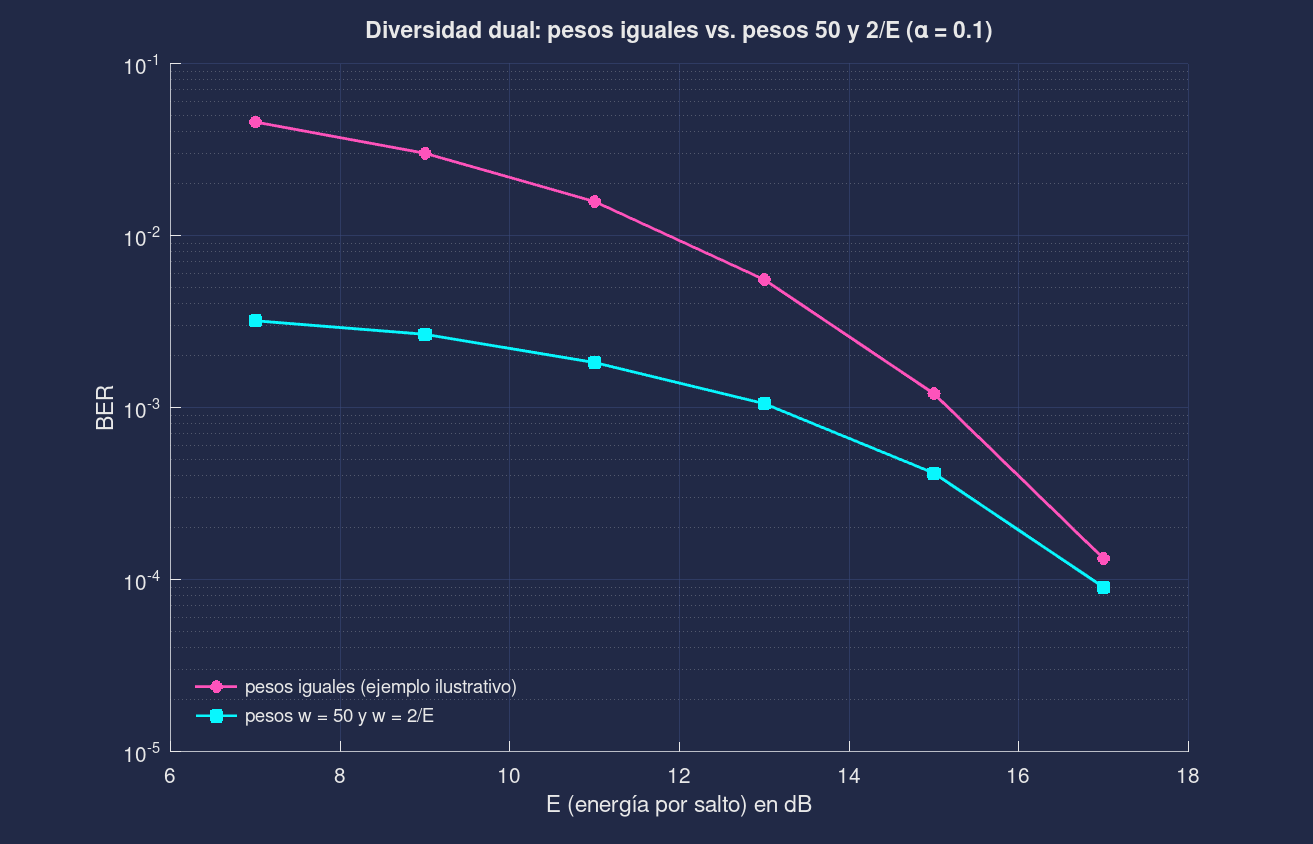
\includegraphics[width=0.9\linewidth]{p11_diversidad.png}
  \caption{Diversidad dual: comparación del combinador de pesos iguales con el
  de pesos $50$ y $2/E$. La ganancia es mayor cuando la energía por salto es
  pequeña.}
  \label{fig:p11}
\end{figure}

\begin{table}[H]
  \centering
  \caption{BER con diversidad dual para los dos esquemas de pesos.}
  \label{tab:p11}
  \begin{tabular}{@{}cccc@{}}
    \toprule
    $E$ (dB) & $E$ & Pesos iguales & Pesos $50$ y $2/E$ \\
    \midrule
    7  & 5.01  & $4.55\times10^{-2}$ & $3.18\times10^{-3}$ \\
    9  & 7.94  & $3.00\times10^{-2}$ & $2.66\times10^{-3}$ \\
    11 & 12.59 & $1.57\times10^{-2}$ & $1.82\times10^{-3}$ \\
    13 & 19.95 & $5.52\times10^{-3}$ & $1.05\times10^{-3}$ \\
    15 & 31.62 & $1.20\times10^{-3}$ & $4.14\times10^{-4}$ \\
    17 & 50.12 & $1.32\times10^{-4}$ & $9.00\times10^{-5}$ \\
    \bottomrule
  \end{tabular}
\end{table}

\paragraph{Discusión.} Con información del estado de interferencia, el
combinador puede casi descartar el salto contaminado y quedarse con el salto
limpio; sin esa información, el promedio de un salto bueno y uno malo arrastra
el ruido del interferido. La mejora es grande precisamente donde la energía por
salto es pequeña, que es el régimen en el que la interferencia domina. El precio
es la necesidad de estimar en el receptor qué saltos fueron interferidos
(AGC, detección de energía o información lateral), y de una escala fija que
evite dividir entre cero cuando $\sigma^2=0$.

\paragraph{Código.}
\listado{problema11.m}

% ------------------------------------------------------------- conclusiones
\section{Conclusiones}

\begin{enumerate}
  \item En un canal AWGN, el espectro disperso no mejora la BER referida a
        $E_b/N_0$: la curva de DS/SS coincide con la de BPSK. La ganancia de
        procesamiento aparece cuando la BER se refiere al SNR del canal
        (problema 3) o cuando existe interferencia (problema 2).
  \item Un sistema LPI puede operar con $P_S/P_N=-5$ dB y alcanzar
        $P_e\approx2\times10^{-4}$ gracias a 13 dB de ganancia de procesamiento;
        la señal es invisible en el tiempo pero el correlador la recupera.
  \item Las secuencias-$m$ tienen autocorrelación de dos valores con lóbulo
        lateral $-1/L$ ($-72$ dB para $m=12$), lo que las hace ideales para
        sincronización. Combinar secuencias de periodos distintos no conserva
        esa propiedad: el compuesto de $m=3$ y $m=4$ tiene lóbulos de $-1/7$.
  \item Las secuencias Gold de 31 chips presentan tres valores de
        autocorrelación ($-9/31$, $-1/31$ y $7/31$) y una correlación cruzada
        máxima de $9/31$; son un compromiso entre autocorrelación y tamaño de la
        familia.
  \item En CDMA síncrono las correlaciones cruzadas a retardo cero valen
        $-1/31$, así que cuatro usuarios se comportan como uno solo. El
        asincronismo convierte esas correlaciones en parciales (hasta $9/31$) y
        produce un piso de BER de $10^{-3}$ a $10^{-2}$, 42 veces peor a 9 dB.
  \item Un LFSR de 7 etapas selecciona las 127 bandas de un sistema FH como una
        permutación; cada banda contiene dos tonos FSK ortogonales separados
        $1/T_b$.
  \item La interferencia de banda parcial con $\alpha=0.1$ es mucho más dañina
        que la de banda completa: la BER decae como $\exp(-\alpha E_b/2J_0)$ y
        requiere 13 dB adicionales para bajar un factor $e$.
  \item La diversidad dual con pesos adaptativos reduce la BER hasta 14 veces
        respecto al combinador de pesos iguales cuando la energía por salto es
        pequeña, a costa de necesitar información del estado de interferencia.
\end{enumerate}

\begin{thebibliography}{9}
\bibitem{proakis} J. G. Proakis, \emph{Digital Communications}, 4a ed.,
  McGraw-Hill, 2001, cap.~13 (Spread Spectrum Signals for Digital
  Communications).
\bibitem{proakis_salehi} J. G. Proakis y M. Salehi, \emph{Contemporary
  Communication Systems Using MATLAB}, 2a ed., Brooks/Cole, 2000.
\bibitem{notas} V. I. Rodríguez Abdalá, \emph{Notas del curso de Tecnologías
  Celulares}, UAZ, 2026.
\end{thebibliography}

% ------------------------------------------------------------- apendice
\appendix
\section{Funciones auxiliares}
\label{ap:comun}

Todas las funciones viven en \texttt{comun/}. El generador de secuencias-$m$
implementa un LFSR de Fibonacci y recibe los exponentes del polinomio
primitivo; la autocorrelación usa la ecuación~\eqref{eq:autocorr}; el motor CDMA
genera la señal chip por chip y desensancha cada usuario con su código.

\subsection*{Generador de secuencias-$m$ (\texttt{lfsr\_max.m})}
\listado{comun/lfsr_max.m}

\subsection*{Autocorrelación periódica (\texttt{autocorr\_per.m})}
\listado{comun/autocorr_per.m}

\subsection*{Secuencias Gold (\texttt{gold31.m})}
\listado{comun/gold31.m}

\subsection*{Simulación DS/SS (\texttt{sim\_dsss.m})}
\listado{comun/sim_dsss.m}

\subsection*{Simulación CDMA (\texttt{simular\_cdma.m})}
\listado{comun/simular_cdma.m}

\subsection*{Función $Q$ (\texttt{qfunc.m})}
\listado{comun/qfunc.m}

\section{Cómo reproducir los resultados}

Desde la carpeta \texttt{Tareas/tarea2/}:
\begin{center}
\begin{tabular}{@{}ll@{}}
  \toprule
  Acción & Comando \\
  \midrule
  Un problema & \texttt{octave --no-gui problema01.m} \\
  Todos & \texttt{./ejecutar\_todo.sh} \\
  Reporte & \texttt{latexmk -pdf main.tex} \\
  \bottomrule
\end{tabular}
\end{center}

Cada script escribe su figura en \texttt{figs/} y sus números en
\texttt{datos/problemaNN.txt}. Las semillas están fijas, de modo que una nueva
corrida reproduce las mismas cifras. Los resultados también se pueden obtener
con MATLAB sin cambios: se usan únicamente funciones básicas
(\texttt{rand}, \texttt{randn}, \texttt{fft}, \texttt{kron}, \texttt{stem},
\texttt{semilogy}).

\end{document}
